% last updated in April 2002 by Antje Endemann
% Based on CVPR 07 and LNCS, with modifications by DAF, AZ and elle, 2008 and AA, 2010, and CC, 2011; TT, 2014; AAS, 2016

\documentclass[runningheads]{llncs}
\usepackage{graphicx}
\usepackage{caption}
\usepackage{amsmath,amssymb} % define this before the line numbering.
\usepackage{ruler}
\usepackage{color}
\usepackage{array}
\usepackage{cite}

\usepackage{caption} 
\captionsetup[table]{skip=3pt}

\newcommand{\etal}{\mbox{\emph{et al.\ }}}

\usepackage[width=122mm,left=12mm,paperwidth=146mm,height=193mm,top=12mm,paperheight=217mm]{geometry}

\makeatletter
\newcommand{\thickhline}{%
    \noalign {\ifnum 0=`}\fi \hrule height 1pt
    \futurelet \reserved@a \@xhline
}
\newcolumntype{"}{@{\hskip\tabcolsep\vrule width 1pt\hskip\tabcolsep}}
\makeatother

\begin{document}

\pagestyle{headings}
\mainmatter
\def\ECCV16SubNumber{***}  % Insert your submission number here

\title{Joint Event Recognition and Image Selection} % Replace with your title

\titlerunning{ECCV-16 submission ID \ECCV16SubNumber
}

\authorrunning{ECCV-16 submission ID \ECCV16SubNumber}

\author{Anonymous ECCV submission}
\institute{Paper ID \ECCV16SubNumber}


\maketitle

\begin{abstract}
Automatic image organization of personal photos is a problem with many real world applications, and can be divided into two main tasks: recognizing event types of the photo collections, and selecting interesting images from the collections. The two tasks are both challenging, in that the photos from the same event type are highly varied, and there is a great deal of overlap in photos from different event types. In this paper, we looked into the possibility of simultaneously solving both tasks: album-wise event recognition and single image event-specific importance score prediction. We collected an event album dataset with both event type labels and image importance labels, refined from the existing CUFED dataset. We propose a hybrid system consisting of three parts: Siamese network based event-specific image importance prediction, Convolutional Neural Network(CNN) based event recognition, and Long Short-Term Memory(LSTM) based sequence level event recognition, and we propose an iterative updating procedure for event type and image importance score prediction. We show with experiments that the proposed method outperforms the classical approach based on static image classification, and more importantly, we verified that image importance score prediction and event type recognition can in turn help the performance of each other. 


\keywords{Event Recognition, Image Importance, Convolutional Neural Network, Long Short-Term Memory}
\end{abstract}


\section{Introduction}
With the advent of cheap cameras in nearly all of our devices, and automated uploading to the cloud, and practically unlimited storage,
%With the rapid progress in portable photo taking devices and the increasing volume of storage devices and services,
it becomes painless to take photos frequently in daily life, resulting in the explosion of personal photo collections. However, the oversized image collections make it difficult for us to organize the photos, and thus automatic organization algorithms are highly desirable. The organization of personal photo collections can be decomposed into two stages: recognition of the event types of a photo collection, and suggesting the most interesting/important images in the photo collection to represent the album, e.g. making an album cover, or suggesting to the user a set for a further use, e.g. making a photo book. The two stages assist users in keeping the photo collections organized and free of irrelevant images.

Both image importance prediction and event recognition have been studied independently. 

Studies of event recognition can be separated into several types. The most popular branches of study use videos as input \cite{2015trecvidover, TangCVPR12, xu2015discriminative}. Spatial and temporal features of videos are usually used for this task. The success of Long Short-Term Memory (LSTM) networks for sequence tasks have also extended to video based event recogntion. In \cite{lstm}, the LSTM network and visual feature extraction network is stacked, and the network can deal with both event recognition and description. Reiter \etal \cite{lstm2} also combine LSTM and HMMs for video meeting analysis.
% \textcolor{red}{!!!!!} 
At the other end of the spectrum, event recognition for single static images has also been attempted \cite{what_where, Park_2015_CVPR_Workshops, cSalvadora}. In contrast to video based event recognition, there is no temporal information to exploit, and there is no need to consider relevant frame importance or contribution to the event, since there is only one ``frame." This problem can be viewed as a special case of scene recognition, and both object level features and scene level features are utilized \cite{what_where}. The recent success of Deep Neural Networks, especially  Convolutional Neural Networks(CNN) provides us with an outstanding visual representation, that can be used for the single static image event recognition task \cite{Park_2015_CVPR_Workshops, cSalvadora}. 

Album-wise event recognition lies in the middle between single-image-based and video-based event recognition. Images in an album can be thought of a very sparse samples from the event video. Photo albums differ from videos in that consecutive images from the photo album are no longer continuous, and can have very different visual and semantic information. However, there is still sequential information in time-stamped albums, and the images in an album are of varied importance. In \cite{HMM}, an HMM-based model is proposed to use the sequential information in albums for the recognition task. It wss shown that the temporally-sensitive HMM outperforms the simple aggregation of predictions from all the images in an album. This indicates that the sequential information in an album is helpful for  album-wise event recognition.

Image importance is a complex image property which is related to various factors, such as aesthetics \cite{aesthe_14}, interestingness \cite{interesting} and image memorability \cite{Isola2011}. It has been shown \cite{CVPR} that importance of an image is modulated by the context of the image, making image importance album-dependent, or event-specific. Event-specific image importance is a highly subjective judgment, and learning it is a very challenging task, due to the very high intra-class variability, and the underlying uncertainty caused by the subjectiveness of the property. Nevertheless, it is still possible to predict it. 

Returning to the task of photo collection organization, we ask the question: can we simultaneously recognize the event type for an album, and discover important images in the event album? To answer this question, this paper makes the following contributions: 1. We refine the existing event curation dataset CUFED by collecting more human annotations for album event types for more reliable ground-truth, and allow for multilabel annotation for an album. The multilabel and ground-truth ambiguity between event types provides us with more training information, and allows for a fairer evaluation at the testing stage; 2. We propose a joint event recognition/image importance prediction algorithm. We use a CNN for image level event recognition, and a Siamese Network for event-specific image importance prediction. An iterative update scheme is conducted during the test stage, and we find that event recognition and image importance prediction can improve each other's performance; 3. We further boost the performance of event recognition with an LSTM network that leverages sequence information in labeling the album.

\section{Related Works}
Our work is partly inspired by \cite{CVPR}, who proposed a novel image property: event-specific image importance. In this work, it is claimed that image importance or interestingness is contextual and is related to the album it is in. For example, a photo of a beautiful work of architecture is important in an album of an urban trip, yet not so important in a wedding event.  A Siamese network is used to predict the relative score difference between an input image pair, and is 
 jointly trained on all event types.
However, in this work, the event-specific image importance score is predicted given the ground-truth event type of the album. In our work, we extend this idea to training a system simultaneously for event recognition and importance image curation, so that additional user input of event type for testing is not required.

Our work is closely related to the study of event recognition for a personal album. The model in \cite{Mattivi11} classifies a personal album into 8 social events and 10 sports events simply by aggregating the SVM classification result from single images in the album. In \cite{pattern}, Tsai \etal exploit object level patterns for event type recognition. Object patterns are learnt from single images,  and then an album-wise SVM is trained on the frequency distribution of different object patterns appearing in an album. Similarly, Imran \etal \cite{Imran09} use the Pagerank technique to mine the most useful features for an event, and an album-wise SVM classifier is used for recognitoin.
The above works treat albums as an unordered collection of images. On the other hand, in \cite{HMM}, Bossard \etal exploit the sequential nature of personal albums and use an HMM based sub-event approach for event recognition. They use temporal sequence of the images, and model an album with successive latent sub-events to boost the recognition performance.  They collected a 14 class dataset consisting of 807 albums for the task. 

Event recognition for single photos has also been studied.  Li \etal \cite{what_where} use a generative graphical model to recognize event types of a database with 8 sports events. Their model integrates cues from scene and object categorization to classify the sports events. Salvador \etal\cite{cSalvadora} focus on cultural event recognition. They integrate cues from visual features extracted by a CNN and from the time-stamp of a photo, inspired by the fact that photos of a cultural event are mostly taken in the same period of time. However, in personal photo collections, the relevance of an image within an event album varies a great deal. These approaches for single images are useful, but not sufficient for album-wise event recognition.

Convolutional Neural Network(CNN) methods have greatly boosted performance in image understanding tasks, such as image classification, object detection and scene recognition \cite{imagenet, googlenet, rcnn, places}. Many studies have switched their focus to higher-level image properties, such as event recognition \cite{event_recognition}, semantic segmentation \cite{long_shelhamer_fcn},  multilabel image annotation \cite{tagging}, and image captioning \cite{lrcn}. Long Short Term Memory(LSTM) networks \cite{lstm} have been proposed for sequence prediction and sequence labeling. LSTM networks have advantages over traditional Recurrent Neural Networks (RNN) in that they can maintain contextual information across  an extended sequence of data. LSTMs have achieved success for tasks such as handwritten text recognition \cite{Graves} and speech recognition \cite{speech}. Relevant to our work, the Long-term Recurrent Convolutional Network (LRCN) model \cite{lrcn} has been proposed to stack CNN feature extractor and LSTM networks for sequential learning of videos or images.


\section{The ML-CUFED Dataset}
In order to train and evaluate the joint curation-recognition model, we use the Curation of Flickr Events Dataset (CUFED), and refine it by collecting more human opinions on the event types in the dataset. We can the new dataset MultiLabel-CUFED (ML-CUFED). In this section, we describe the dataset, and provide a consistency analysis of the labels collected from Amazon Mechanical Turk (AMT). The dataset will be made available to the public.
\subsection{The CUFED Dataset}
The CUFED Dataset is an image curation dataset extracted from the Yahoo Flickr Creative Commons 100M Dataset (YFCC100M). 20,000 albums were segmented by user tags and timestamp, and then their event types were collected from workers on AMT. Each album received 3 workers' labels. The dataset contains 23 most common event types from our daily life, ranging from nature trips to weddings. For each event type, 50-200 albums are further randomly sampled from the 20,000 albums, forming the CUFED dataset of 1883 albums. The importance score for each image in the albums was then decided by workers from AMT. The final ground-truth event-specific importance scores of the images were obtained from the average of 5 workers' votes.

One problem the CUFED Dataset has is that the event type of an album is decided by only three workers, andthe workers were constrained to give a single label to each album. However, for an album with ambiguous event types or with multiple event types, it is overly restrictive to give the album a single event label. For example, the two albums in Fig~\ref{album} are both birthday events, but they can also fall into the category of casual family/friends gathering. Those two event types are not mutually exclusive. Moreover, intuitively, we would say the album on the right is a more typical birthday event, with most images focusing on the little boy celebrating his birthday, while the album on the left is more of a casual family/friends gathering rather than an obvious birthday event. Therefore, collecting the event types and their proportion in one album from multiple people's view is necessary. This results in a multi-label event recognition dataset with richer information. 
\begin{figure}
\centering
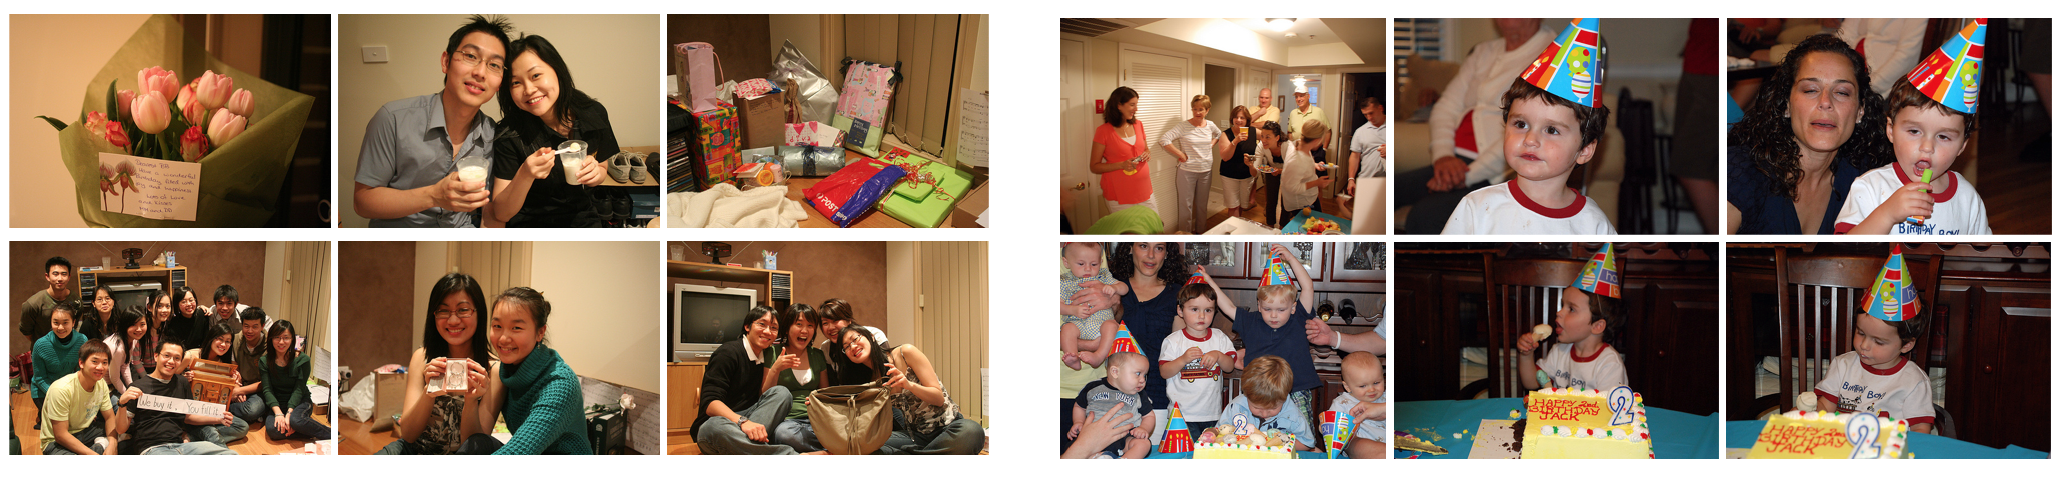
\includegraphics[width=4.5in]{album}
\caption{Example of two birthday albums (both have the photo uploader's tag ``birthday"). }
\label{album}
\vspace{-0.15in}
\end{figure}




\subsection{Data collection}
On top of the three votes the dataset already has, we collected 9 more workers' opinions, and allowed for multiple choices for each album. One worker could select up to three event types for an album. There were totally 299 distinct workers who participated in the task.

The quality of different AMT workers' submissions vary. Therefore, we need to do quality control in order to collect high quality annotations. Before the real task, only workers who passed an album event recognition test (which is very similar to the actual task) were allowed proceed to work on the actual task. During the tasks, there was another round of quality control. After workers submitted the tasks, the results they turned in were compared with other workers' submissions, and submissions that highly diverged from others were further manually inspected. If the divergence was unreasonable, the submission was rejected. After all the annotations from workers were collected, we further cleaned the annotations by eliminating the labels with minor votes: for each album, all the event types with only one vote were discarded. 

For the final ground-truth event types and their proportion of one album, we use the the proportion of votes among all the votes. For workers who gives votes to more than one label, each of the votes he or she gives is normalized so that all the votes sum to one.

\subsection{Dataset Analysis}
To check the validity of the dataset we collected, we analyzed the annotations in several ways. Each album can between 9 and 27 votes (because we allow for multiple choices from one worker). 76\% of the albums received votes for two or fewer event types. This suggests the high coherence of those albums. 95\% of the albums received votes for three or fewer event types.  To check the consistency among workers, we randomly split the 299 workers into two halves, and for each album we checked whether the annotations from one half was consistent with the other half. For each album, we examined whether the top event types suggested by these two independent groups were the same.
We repeated the random split 100 times, and on average, for 89.6\% of the albums, the event type receiving most votes were the same for both groups. This suggests that despite the ambiguity of some album types, we got consistent opinions from different AMT workers. 

\section{Approach}
\label{approach}
In this section, we describe our approach to jointly attain image importance prediction and album event-type recognition. The system is shown in Figure~\ref{figure1}. 

\begin{figure}
\centering
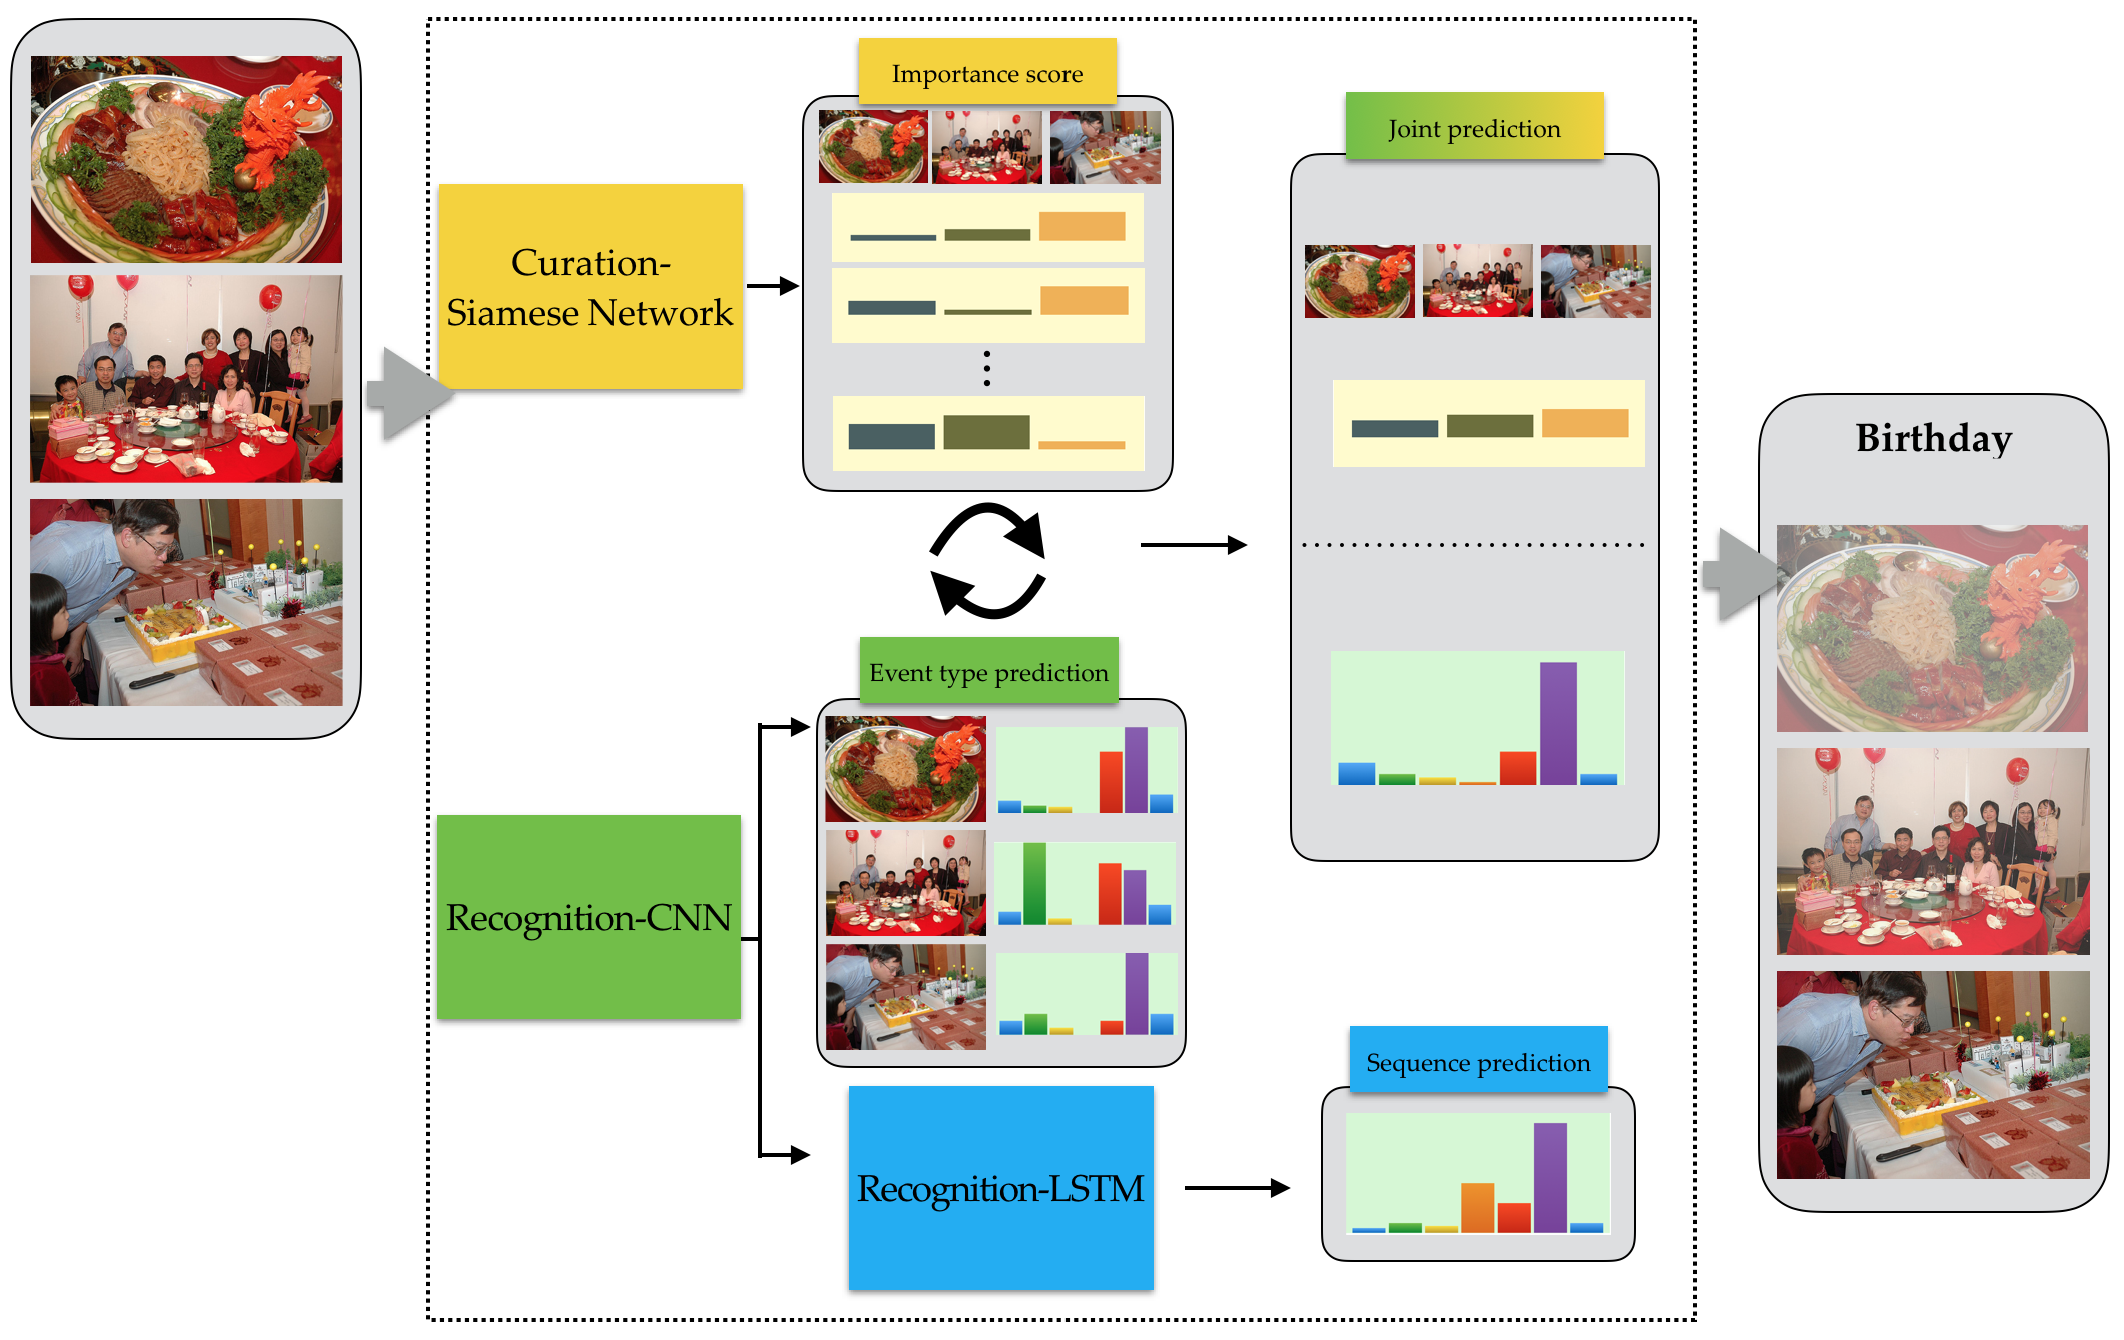
\includegraphics[width=4.8in]{architecture}
\caption{The joint album recognition-curation system. The system consists of three parts: a Siamese network for image importance score prediction, a CNN for single image event-type recognition, and a LSTM network for album event-type recognition. During the test stage, the three components interact and jointly produce the prediction of album event type and image importance score.}
\label{figure1}
\vspace{-0.3in}
\end{figure}

\subsection{Event curation network}
\label{curation_section}
%\textcolor{red}{Not sure how detailed should  the part of previous paper be.}

For event curation purposes, we followed the approach in \cite{CVPR}, using Piecewise Ranking (PR) loss to jointly train a Siamese network to predict the importance score difference between an image pair given the ground-truth event type of the input image pair. The architecture can predict the relative event-specific importance score for a set of images, and is found to perform better than a traditional CNN that directly predicts the absolute important score of an image.
One difference between our implementation and \cite{CVPR} is that the ground-truth event type for the input image pair  is not a one-hot representation; instead, the ground-truth event type label is a soft distribution. The event type label is used to gate the output and gradient of the Siamese network: for an input image pair of a certain event type $c \in C$, only the part of the network which corresponds to event type $c$ is back-propagated.  Here, to train the Siamese network on the multi-event type label, we change the 0/1 gating to a soft gating, thus for an input image pair with multiple event type labels, the error signals from all the possible labels are back-propagated, but with a weight: the ground-truth probability of that event type. Another scheme is to still use 0/1 gating, but for an input image pair with multiple event type labels, there is equal probability for the network to view the input image pair as from one of the possible labels. This gives more relaxation on the ground-truth event type label.
\subsection{Event recognition network}
One of the properties of  an ``event album" that makes it different from a simple collection of images is that it is a sequence, and this provides us with the temporal relationship between the images. LSTMs have been successfully applied to sequential tasks, and its ability to do long-range context memorization is suitable for our task of album-wise event recognition. Therefore, we use the LSTM network to capture the sequential information, in addition to a classical CNN that captures the visual features of a single image. 

We start with a CNN pre-trained on ImageNet \cite{caffe} \cite{imagenet}, and fine-tune it on the CUFED Dataset to recognize a single image's event type. We then extract the high level CNN features for each image from the adapted network, and use them as the input features to train the LSTM network for album-wise event recognition. The LSTM network consists of a single LSTM layer, a mean pooling layer, and a softmax prediction layer. 

The target for both fine-tuned the CNN and the LSTM network is the soft distribution of the ground-truth event labels. Again, another scheme is to use the one-hot target, but treat each training example as from one of the possible event types with equal probabilities. 
\textcolor{red}{FROM GARY. WE WILL PROVIDE BOTH APPROACH IN THE RESULTS PART. AND ACTUALLY THE SECOND APPROACH HAS A LITTLE BETTER RESULT. Another approach would be to train each album multiple times, with different event labels each time. We deemed this approach to be less elegant than using the distribution as the target.}


During the testing stage, the album-wise prediction from the LSTM network and the image-wise prediction from the CNN are combined to produce the final prediction for the album type. 

\subsection{The iterative curation-recognition procedure}
For an ``event album", more interesting images or important images give us more information about the event type of this album. For example, although a candle blowing image may only appear in an album once, it is very helpful for deciding the event type of the album. However, as shown in \cite{CVPR}, the importance of an image is related to the context it is in, and is event-type dependent. Therefore, we propose that the image importance score can help with event recognition of an album, while event recognition of an album will in turn improves the image importance score prediction.

We denote an $N$-image album as $\mathbf{S}= \left \{I^{1}, ..., I^{N}  \right \}$. From the event curation network in Section~\ref{curation_section}, we obtain the importance score of an image $I^{n} \in S $ given its event type: $W^{n}= \left [w_{1}^{n} , ..., w_{C}^{n}  \right ]^{T}$ where $C$ is the number of event types. From the event recognition CNN, we can also get the prediction of the event type for a single image $P^{n}= \left [ p_{1}^{n} , ..., p_{C}^{n}  \right ]^{T}$. We then conduct the iterative curation-recognition procedure:
\begin{equation}
\left\{\begin{matrix}
Q(k+1) = \left [ P^{1}, P^{2}, ..., P^{N} \right ] \cdot V(k)^{\alpha }\\ 
V(k+1) = \left \{[W^{1}, W^{2}, ..., W^{N}]^{T}\circ\textup{I}\left \{ p^{n}_{c}\geq m \cdot \max_{c'}(p^{n}_{c'}) \right \}_{n,c}\right \} \cdot  Q(k+1)
\end{matrix}\right.
\label{eq1}
\end{equation}

Or equivalently, it can be written in vector form:
\begin{equation}
\left\{\begin{matrix}
q_{c}(k+1) = V^{T}(k)^{\alpha }\cdot  P^{n}\\ 
v^{n}(k+1) = \left \{W_{n}^{T} \circ \textup{I}\left \{ p^{n}_{c}\geq m\cdot \max_{c'}(p^{n}_{c'}) \right \}_{(c,1)}\right \} \cdot  Q(k+1)
\end{matrix}\right.
\end{equation}

where the $N$-dimensional column vector $V(k) = [v^{1}, ..., v^{N}]^{T}$ is the $k$-th step prediction for all images' importance score in album $S$, and the $C$-dimensional column vector $Q(k) = [q_{1}, q_{2},..., q_{C}]^{T}$ is the $k$-th step prediction for the album's event type.

$\textup{I}\left \{ p^{n}_{c}\geq m\cdot \max_{c'}(p^{n}_{c'}) \right \}_{n,c}$ denotes the binary mask that eliminates the event type predictions with low confidence, and makes sure only event types with high probability contribute to the image importance prediction. 
%$m_{1}$ is the threshold to only allow for important images to contribute to event type prediction of the album. 
$\alpha$ is the weight factor that reflects our emphasis on the image importance score.

By iteratively conducting the procedures in Equation~\ref{eq1}, we obtain the album-wise event prediction $Q$ and image importance score prediction $V$. 

Note that Equation~\ref{eq1} is not guaranteed to converge. In the case of oscillation between states, we set a maximum number of iterations, and when the iteration number hits the threshold,  predictions for $Q$ and $V$ are obtained by averaging over the three previous steps.
\subsection{Joint prediction}
The iterative curation-recognition procedure takes image importance into account for event type prediction, while the LSTM network is trained to do the same task, taking the sequence of images into account. These two processes stress two distinct properties of  event albums, and are complementary to each other. Therefore, we average the predicted probability density from the LSTM network $Q_{LSTM}$ and from the iterative curation-recognition procedure $Q_{iter}$, and get the final event type prediction for an album. The entire system is illustrated in Figure~\ref{figure1}.

\section{Experiments}
In this section, we evaluate our approach for both event recognition and image importance prediction on ML-CUFED Dataset, and we compare our event recognition result with \cite{HMM} on PEC Dataset.
\subsection{Baselines}
Our joint recognition-curation method produces two parts of result: album event recognition, and image event-importance prediction. 
For event recognition, we compare our result with the baseline by training a single CNN to classify each input image into event types. We denote this method CNN-recognition. In addition, when our algorithm moves on, the intermediate result can also be compared with the final result. Therefore, we compare our method with the following methods:
\begin{itemize}
  \item \textbf{CNN-recognition}: Use a single CNN to predict event type for a single image. To predict the event type of one album, predictions of all the images are averaged.
  \item \textbf{CNN-Iterative}: Use the recognition prediction from the CNN-recognition network and the image prediction result from Siamese Network to joint obtain the modified recognition prediction, as described in Section~\ref{approach}.
  \item \textbf{CNN-LSTM}: Use the feature extracted from CNN-recognition as input to an LSTM network, and directly predict the album event type given the input image sequence.
  \item \textbf{CNN-Iterative-LSTM}: our method.
\end{itemize}

To evaluate our image importance prediction result, we provide comparison with several baselines:
\begin{itemize}
  \item \textbf{CNN-Noevent}: Train a Siamese Network to predict the importance score difference of an input image pair. No event type information is given to the network while training or testing. All albums are viewed as from the same ``hyper" event type.
  \item \textbf{CNN-Noevent(test)}: When training the Siamese Network, use the ground-truth event type information to gate the output error and back-propagation signal. In this way, features for each event type are learned separately. When testing, given an image, average the predicted importance score for all possible event types.  
    \item \textbf{CNN-Iterative}: Our method.
    \end{itemize}

\subsection{Experimental Details}
\subsubsection{Dataset.} For ML-CUFED Dataset, we split the albums to training:test 4:1. The test set has 368 albums. To decide the hyper-parameters $(\alpha, m)$ in our iterative model, a validation set with 119 albums is separated from the training set.  For the PEC Event Recognition Dataset \cite{HMM}, we use directly the test set consisting of 10 albums each event type as described in the paper \cite{HMM}, so that we can directly compare our methods.

\subsubsection{Parameter setting}. For both the CNN-recognition network and the Siamese network, we use the 8-layer AlexNet \cite{imagenet} pretrained on ImageNet as the starting point, and fine-tune it on ML-CUFED Dataset. We use similar training scheme with \cite{caffe}, while using a lower learning rate of 0.001. For the LSTM network, we use the 7th layer feature from trained CNN-recognition as the input. The 7th layer feature is 4096-dimensional. and we reduce it to 128-dimensional with PCA. For the LSTM network, we use AdaDalta as optimization method \cite{adadelta} \cite{theano1} \cite{theano2}. For the Siamese network, we follow the settings in \cite{CVPR} and choose the two thresholds as $m_{s} = 0.1$ and $m_{d}=0.3$. For the maximum number of iterations we allow in the joint recognition-curation stage, we us the maximum iteration number 10.

\subsubsection{Evaluation.} For event recognition, we use two methods to evaluate different methods: average accuracy and $\textup{F}_{1}$ Score. For image importance prediction, we follow the evaluation metrics in \cite{CVPR}, using MAP@I$t\%$) and Precision P@($t\%$).  Precision is calculated as the ratio between the number of retrieved relevant images and the number of all relevant images. MAP is the averaged area under the precision-recall curve, and can be calculated:
\begin{equation}
\textup{AP(S)}@t\%=\int_{0}^{1}p(r)d(r)\approx \frac{\sum_{k=1}^{n}p(k)\times \textup{rel}(k)}{\left \lceil n\cdot t\% \right \rceil}
\end{equation}
\begin{equation}
\textup{MAP(U)}@t\% = \frac{1}{N}\sum_{i=1}^{N}\textup{AP}(\textup{S}_{i})@t\%
\end{equation}


\subsection{Results on ML-CUFED Dataset}
\subsubsection{Event-specific image importance}

For the event-specific image importance score prediction task, we provide the comparison of our methods with baselines in Table~\ref{aesthetic_table}. To show the upper-bound of our method, we also show the result for CNN-Cheating: It is achieved supposing we know the actual event types of each test album, and use the predicted importance score for that ground-truth event type as the prediction. Note that in our setting we assume only albums are given, and no additional information is added. Therefore, the result of CNN-Cheating here just serves as the best we can get if the event recognition stage is perfect. Our CNN-Cheating result is very similar to that achieved in \cite{CVPR}. As shown in Table~\ref{aesthetic_table}, CNN-Noevent performs a little better than CNN-Noevent (test). This suggests the great deal of divergence of the importance prediction for different event types. CNN-Iterative outperforms CNN-Noevent greatly, with a steady 3\% MAP increment. There is also a steady 3\% increment for $\textup{P}$ at $t<20\%$.

CNN-Iterative greatly reduces the performance loss from knowing the event types (CNN-Cheating) to not knowing the event types (CNN-Noevent). 
\begin{table}[]
\centering
\scalebox{0.9}{
\begin{tabular}{c|cccccc|cccccc}
\thickhline
          & \multicolumn{6}{c|}{$\mathbf{MAP}@\mathbf{t\%}$}          & \multicolumn{6}{c}{$\mathbf{P}@\mathbf{t\%}$} \\ \thickhline
t\%       & 5     & 10    & 15    & 20    & 25    & 30    & 5  & 10  & 15 & 20 & 25 & 30 \\ \hline
Random & 0.113 & 0.161 & 0.211 & 0.256 & 0.303 & 0.350 & 0.044  &  0.090   &  0.142  &  0.193  & 0.243   & 0.298   \\
CNN-Noevent(test) & 0.251 & 0.303 & 0.358 & 0.414 & 0.462 & 0.508 & 0.142   &  0.211   & 0.284   & 0.335   &   0.384 & 0.436    \\
CNN-Noevent & 0.258 & 0.316 & 0.369 & 0.425 & 0.475 & 0.519  & 0.168   &  0.245   & 0.307   & 0.373   &   0.422 & 0.468 \\ 
CNN-Iterative &0.282&0.350&0.404&0.456&0.503&0.548&0.192&0.282&0.342&0.396&0.445&0.492 \\ \hline
CNN-Cheating &0.305&0.372&0.424&0.476&0.522&0.565&0.218&0.304&0.361&0.417&0.461&0.504 \\ 
\thickhline
\end{tabular}
}
\caption{Comparison of event-specific image importance predictions using different methods. Evaluation metric here is $\text{MAP}@t\%$ and $P@t\%$. We also show Random ranking score as a lower bound. We also provide a CNN-cheating result which uses ground-truth event type information when testing.}
\label{aesthetic_table}
\vspace{-0.35in}
\end{table}


\subsubsection{Event recognition}
Table~\ref{CUFED} shows the results of different methods for event recognition. Note that ML-CUFED allows multiple label, therefore the accuracy here is different from the conventional accuracy: for an album, we only evaluate on top 1 prediction. If the predicted event type is among the ground-truth event label, we deem this album corrected predicted.
As shown, there is more than 4\% performance gain on the average accuracy, and 5\% gain on $F_{1}$ Score, from the baseline CNN-recognition method to our proposed method. We can also observe that both iterative curation-recognition and LSTM method help for the final result. This suggests that both the two types of information in an event album are helpful to decide the event type of this album: image importance information, and album sequential information. \textcolor{red}{f1 later}

\begin{table}[]
\vspace{-0.2in}
\centering
\scalebox{0.9}{
\begin{tabular}{cccc}
\thickhline
\textbf{Method}             & \textbf{Avg. Acc. } & \textbf{$\mathbf{F}_{1}$-Score} \\ \hline
CNN-recognition    & 75.0\%        &   0.665       \\
CNN-Iterative      & 78.0\%         &   0.701       \\
CNN-LSTM               & 76.6\%              &   0.694  \\
CNN-Iterative-LSTM & 79.3\%      &       0.718      \\ \thickhline
\end{tabular}
}
\caption{Comparison of different methods on ML-CUFED Dataset.}
\label{CUFED}
\vspace{-0.4in}
\end{table}


Figure~\ref{confusion} provides the confusion matrix of the baseline CNN-recognition and proposed method CNN-Iterative-LSTM. To allow for multilabel, one test example is on the diagonal of the confusion matrix as long as the top-1 prediction for the album is among the ground-truth event types.
We can observe the great performance gain from baseline method to CNN-Iterative-LSTM. Note though there are two categories with 0\% accuracy: Personal Art Activity, and Personal Musical Activity. This is caused by the intrinsic high ambiguity of these two event types with other event types,  and the lack of training data for these two even types (there are only 23 albums with Personal Music Activity in the entire dataset, and all of them have multiple votes). 


In Figure~\ref{}, we show our event curation and recognition result with a few examples in ML-CUFED Dataset.
\begin{figure}
\vspace{-0.15in}
\centering
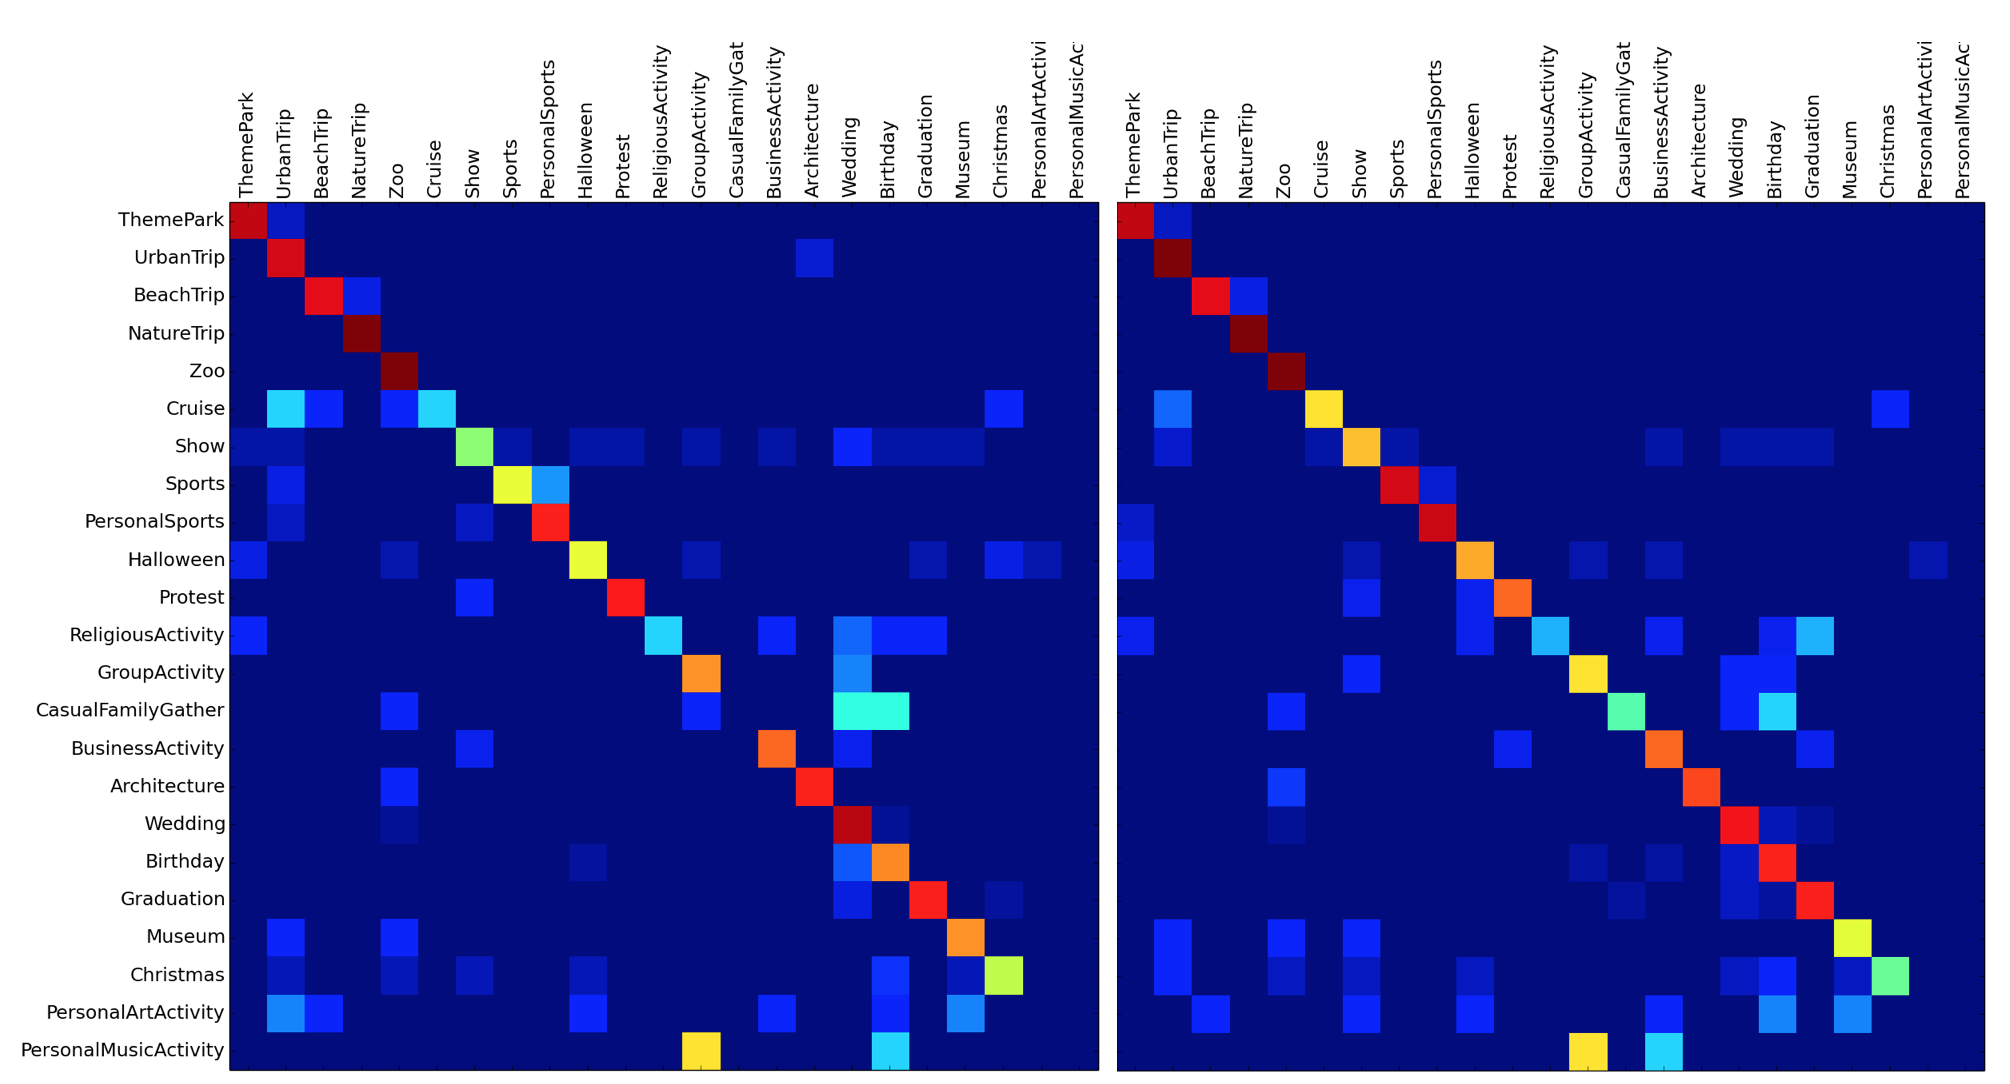
\includegraphics[width=4in]{confusion}
\caption{Confusion matrices for the baseline method(left) and our proposed method(right). \textcolor{red}{ADD NUMBER REDRAW THIS LATER}}
\label{confusion}
\vspace{-0.15in}
\end{figure}


\subsection{Results on PEC Dataset}
\label{PEC_section}
To show the generalization ability of our algorithm, we compare our result with PEC Dataset \cite{HMM}.

The PEC Dataset is an 807-album event dataset, with 14 social event classes. There is no ground-truth importance score labels in PEC, thus we cannot train our algorithm on it. Therefore, we use the model we trained on ML-CUFED and test the model on PEC test set containing 10 albums each class, and compare with the result achieved in \cite{HMM} to make a fair comparison.

In PEC Dataset, there are several event types that are not contained in ML-CUFED, such as Saint Patrick's Day, Easter, and Skiing, and there are multiple event types that can map to single event type in ML-CUFED: Children's Birthday and Birthday can be mapped to single Birthday event in the ML-CUFED dataset. Therefore, we provide the mapping from PEC label to ML-CUFED label in Table~\ref{table1}. Note that the mapping is not perfect. For example, although most albums in Road Trip(PEC) fall into Nature Trip(ML-CU), some of them should fall into Urban Trip(ML-CU), but our mapping ignore this to avoid any bias it might bring to the evaluation. The noise in the mapping makes the performance of our method shown here a little poorer than it really is.

Due to the label changes, we recalculate the performance of Stopwatch HMM (SHMM) \cite{HMM} on the test data. Merged labels are straightforward to deal with, just by merging the two corresponding rows in the confusion matrix. However, for disappeared labels, there are three ways to do: 1. Assume false positive on those labels will be correct predictions if those labels disappear; 2. Assume false positive on those labels will still be incorrect; 3 Ignore false positive on those labels, shrinking the size of the test set. 1 and 2 two extreme ends, being very loose and very strict respectively, while 3 lies in the middle. 

It is also easy to calculate the accuracy of our model: We still take the maximum of predicted probabilities from our model, but ignore those that don't belong in Table~\ref{table1}.

The comparison of different methods is shown in Table~\ref{PEC}. For the result of SHMM, we provide all the three criteria mentioned above. It is worth noting that our networks are fully trained on ML-CUFED, and despite the difference between the two datasets (collected from different sources) and the inevitable label mis-matching, our baseline method (CNN-recognition) already outperforms SHMM. 

\begin{table}[]
\small
\centering
\scalebox{0.9}{
\begin{tabular}{c|c|c|c|cc}
 \thickhline
\textbf{PEC}      & (Children's) Birthday  & Christmas         & Concert & \multicolumn{1}{c|}{Cruise} & Exhibition \\  
\textbf{ML-CUFED} & Birthday                      & Christmas         & Show    & \multicolumn{1}{c|}{Cruise} & Museum     \\ \hline
\textbf{PEC}      & Halloween                     & Hiking, Road Trip & Wedding & Graduation                  &            \\
\textbf{ML-CUFED} & Halloween                     & Nature Trip       & Wedding & Graduation                  &           \\ \thickhline
\end{tabular}
}
\caption{Event type matching from PEC Dataset to ML-CUFED Dataset.}
\label{table1}
\end{table}


\begin{table}[]
%\vspace{-0.2in}
\centering
\scalebox{0.9}{
\begin{tabular}{ccc}
\thickhline
\textbf{Method}             & \textbf{Avg. Acc.} & \textbf{$F_{1}$-Score} \\ \hline
SHMM               & 76.3(1) / 59.1(2) / 72.2(3)\% &  -\\
CNN-recognition    & 80.0\%        &   0.793          \\
CNN-Iterative      & 81.8\%        &   0.813       \\
CNN-LSTM               & 81.8\%              &   0.812  \\
CNN-Iterative-LSTM & 83.6\%      &       0.836      \\ \thickhline
\end{tabular}
}
\caption{Comparison of different methods on PEC Dataset. For the SHMM result, accuracies under three criteria are provided. See Section~\ref{PEC_section} for details.}
\label{PEC}
\vspace{-0.4in}
\end{table}

We show some of the examples of our recognition and event-specific image importance prediction result in Figure~\ref{pec_result}. Although there is no ground-truth labeling for the event-specific importance score for the images, we can look at the sample results qualitatively. From first row in Figure~\ref{pec_result}, we can see that the model does not simply assign a high importance score to the characteristic Christmas tree, but predicts very high score when there are people sitting in front of the Christmas tree. From the second row, we can see the property of the event modulated importance score: although the first image of the beautiful architecture should have high importance in a trip album, in the birthday album, it is much less important even than the table of celebrative food.
\begin{figure}
\centering
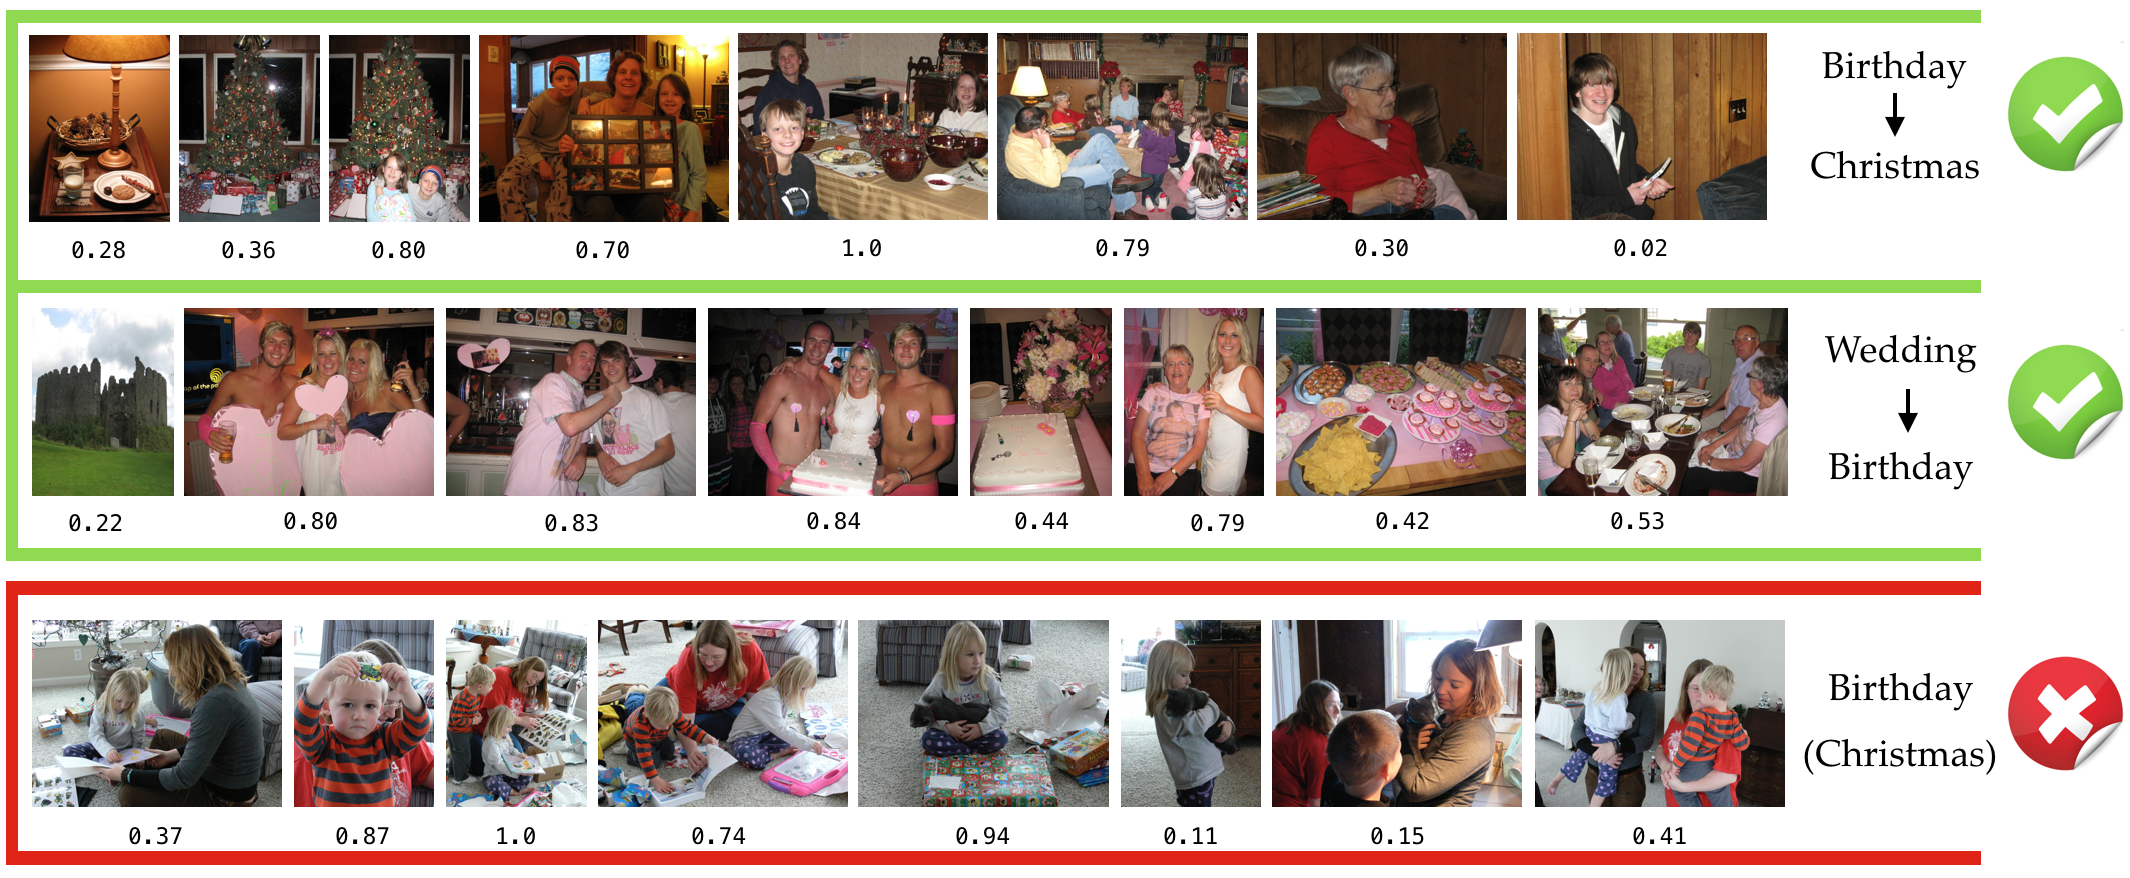
\includegraphics[width=4.8in]{pec_result}
\caption{Some results from PEC Dataset. For first two rows, the prediction from CNN-Direct is wrong as shown in the label above, whereas the sequential information helps the algorithm to modify the final prediction to give the correct answer. For the third row, a case where the model fails to recognize a Christmas event is shown. The predicted important score of each image is shown below the corresponding image. Only a subset of images is shown here for each album due to limited space.}
\label{pec_result}
\vspace{-0.15in}
\end{figure}

\section{Conclusion}
\clearpage

\bibliographystyle{splncs}
\bibliography{egbib}
\end{document}
